\chapter{STXS merging schemes}\label{app:merging_schemes}

\begin{landscape}
\begin{figure}[htbp]
  \centering
  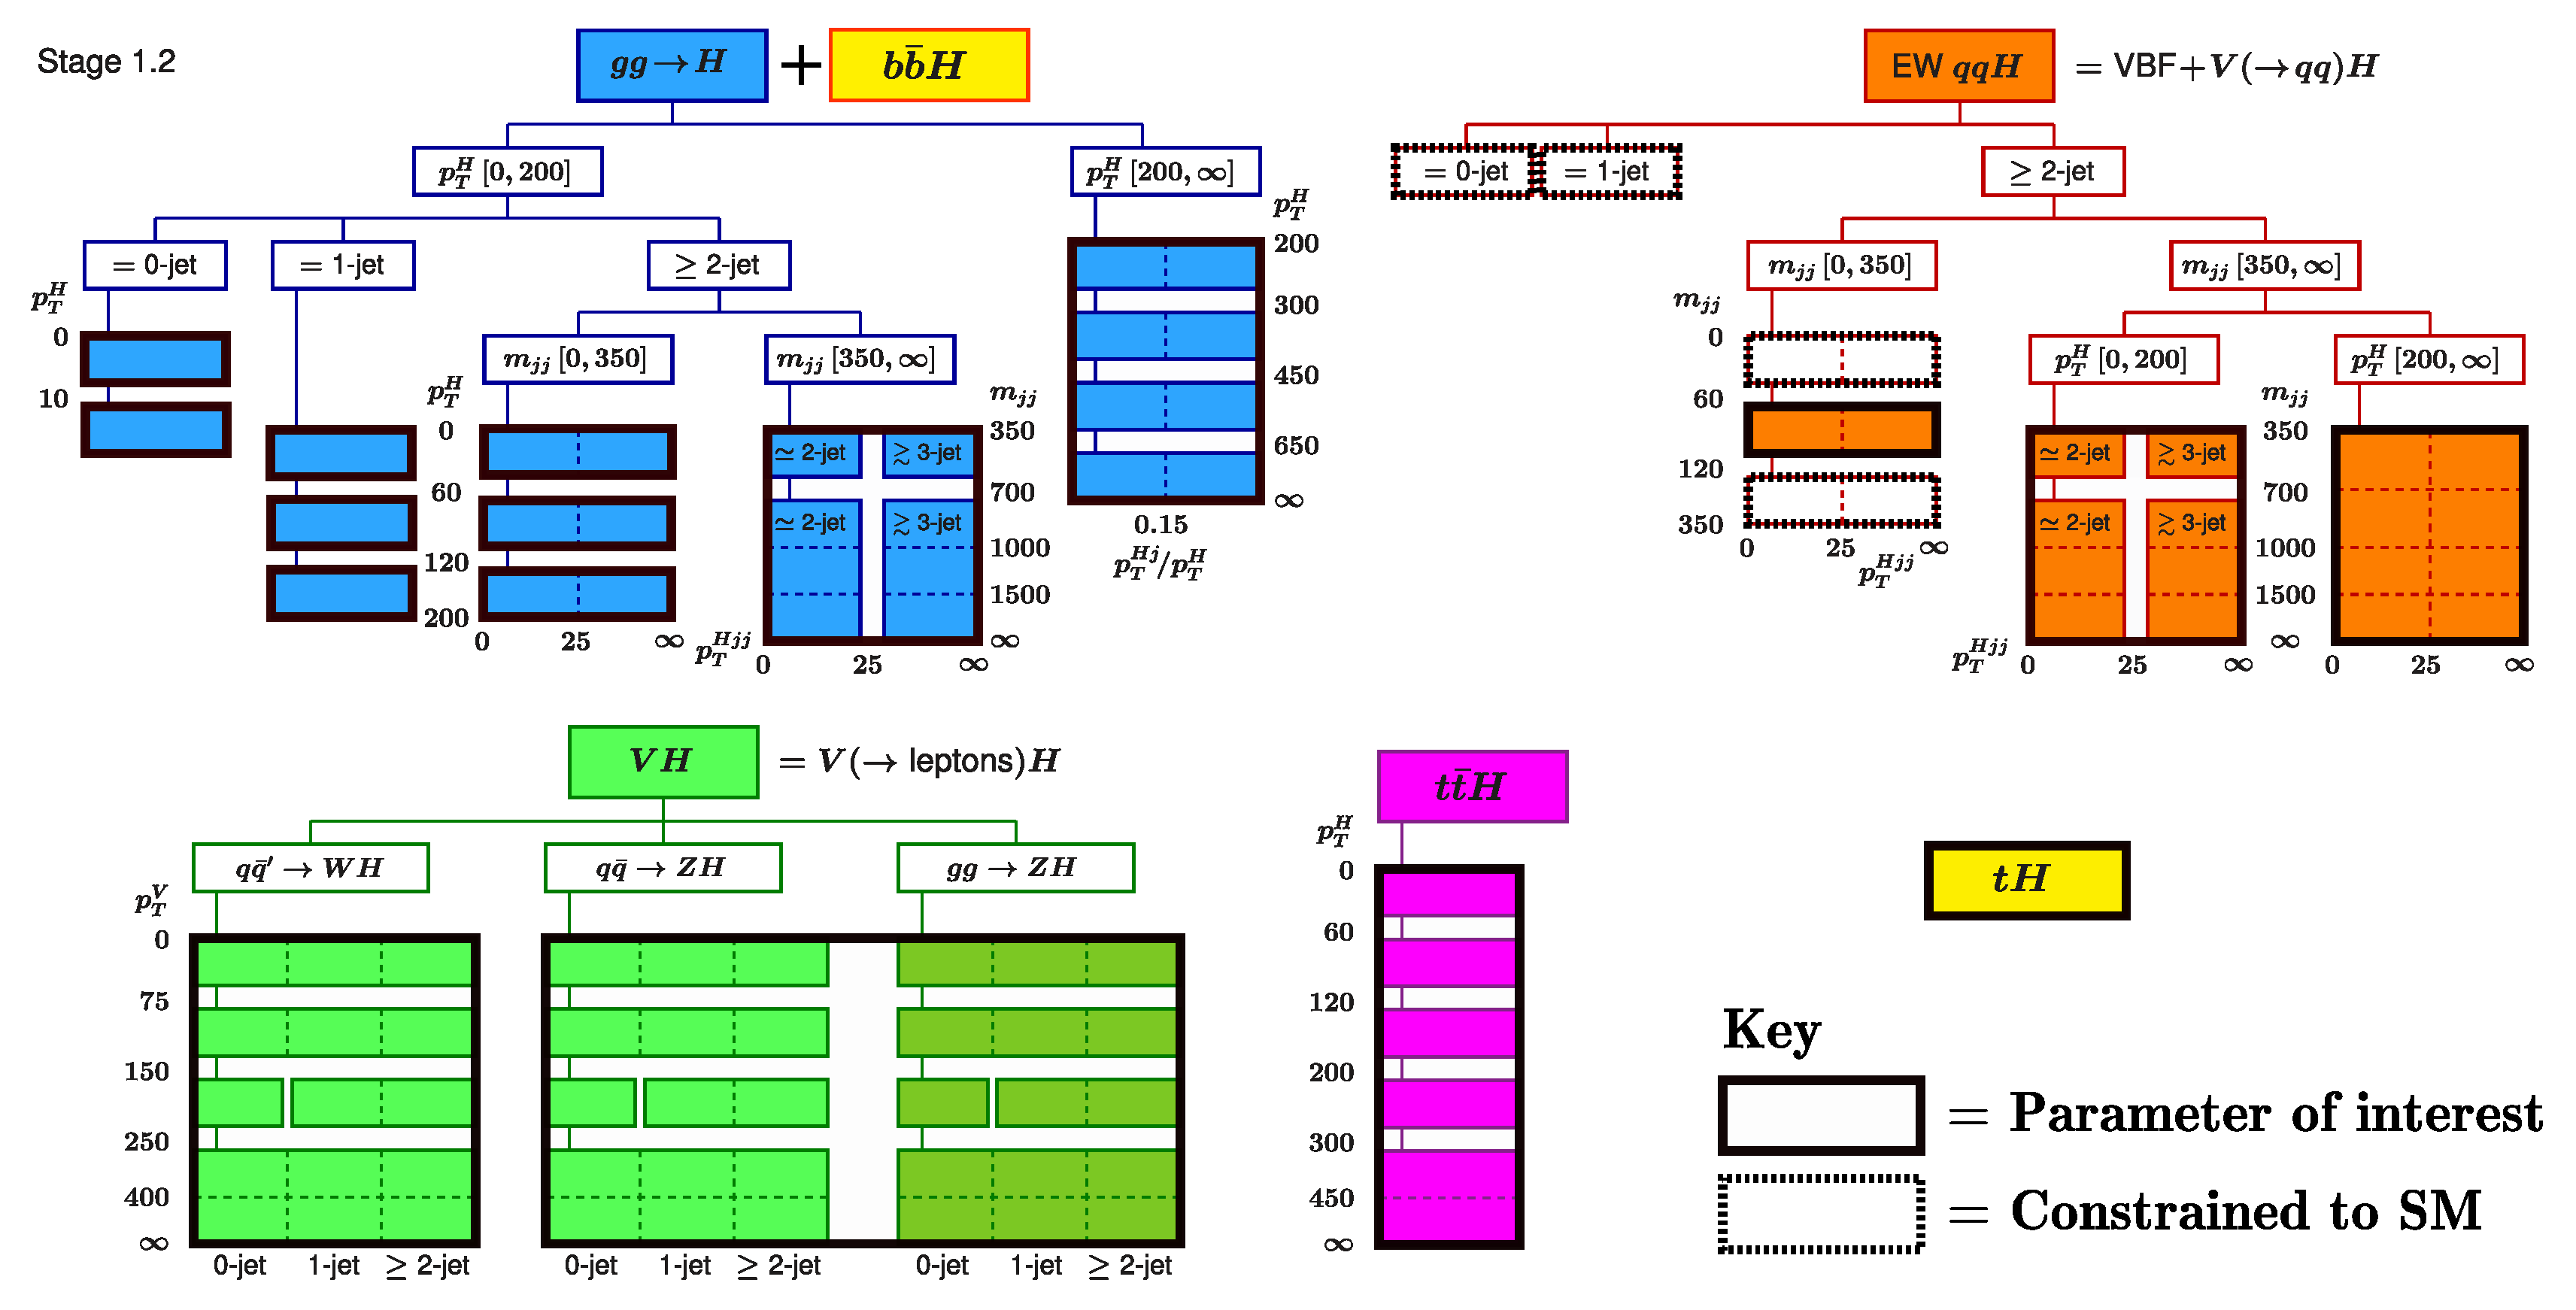
\includegraphics[width=1\linewidth]{Figures/app_merging_schemes/ms_maximal.pdf}
  \caption[Schematic of the maximal merging scheme]
  {
    Schematic to show the maximal merging scheme. The parameters of interest are defined by the solid black boxes, which span over multiple bins for the cases in which the bins are merged. The hatches boxes represent the regions of phase space which are fixed to the SM prediction in the fit. In total 17 parameters of interest are defined.
  }
  \label{fig:maximal_scheme}
\end{figure}
\end{landscape}

\begin{landscape}
\begin{figure}[htbp]
  \centering
  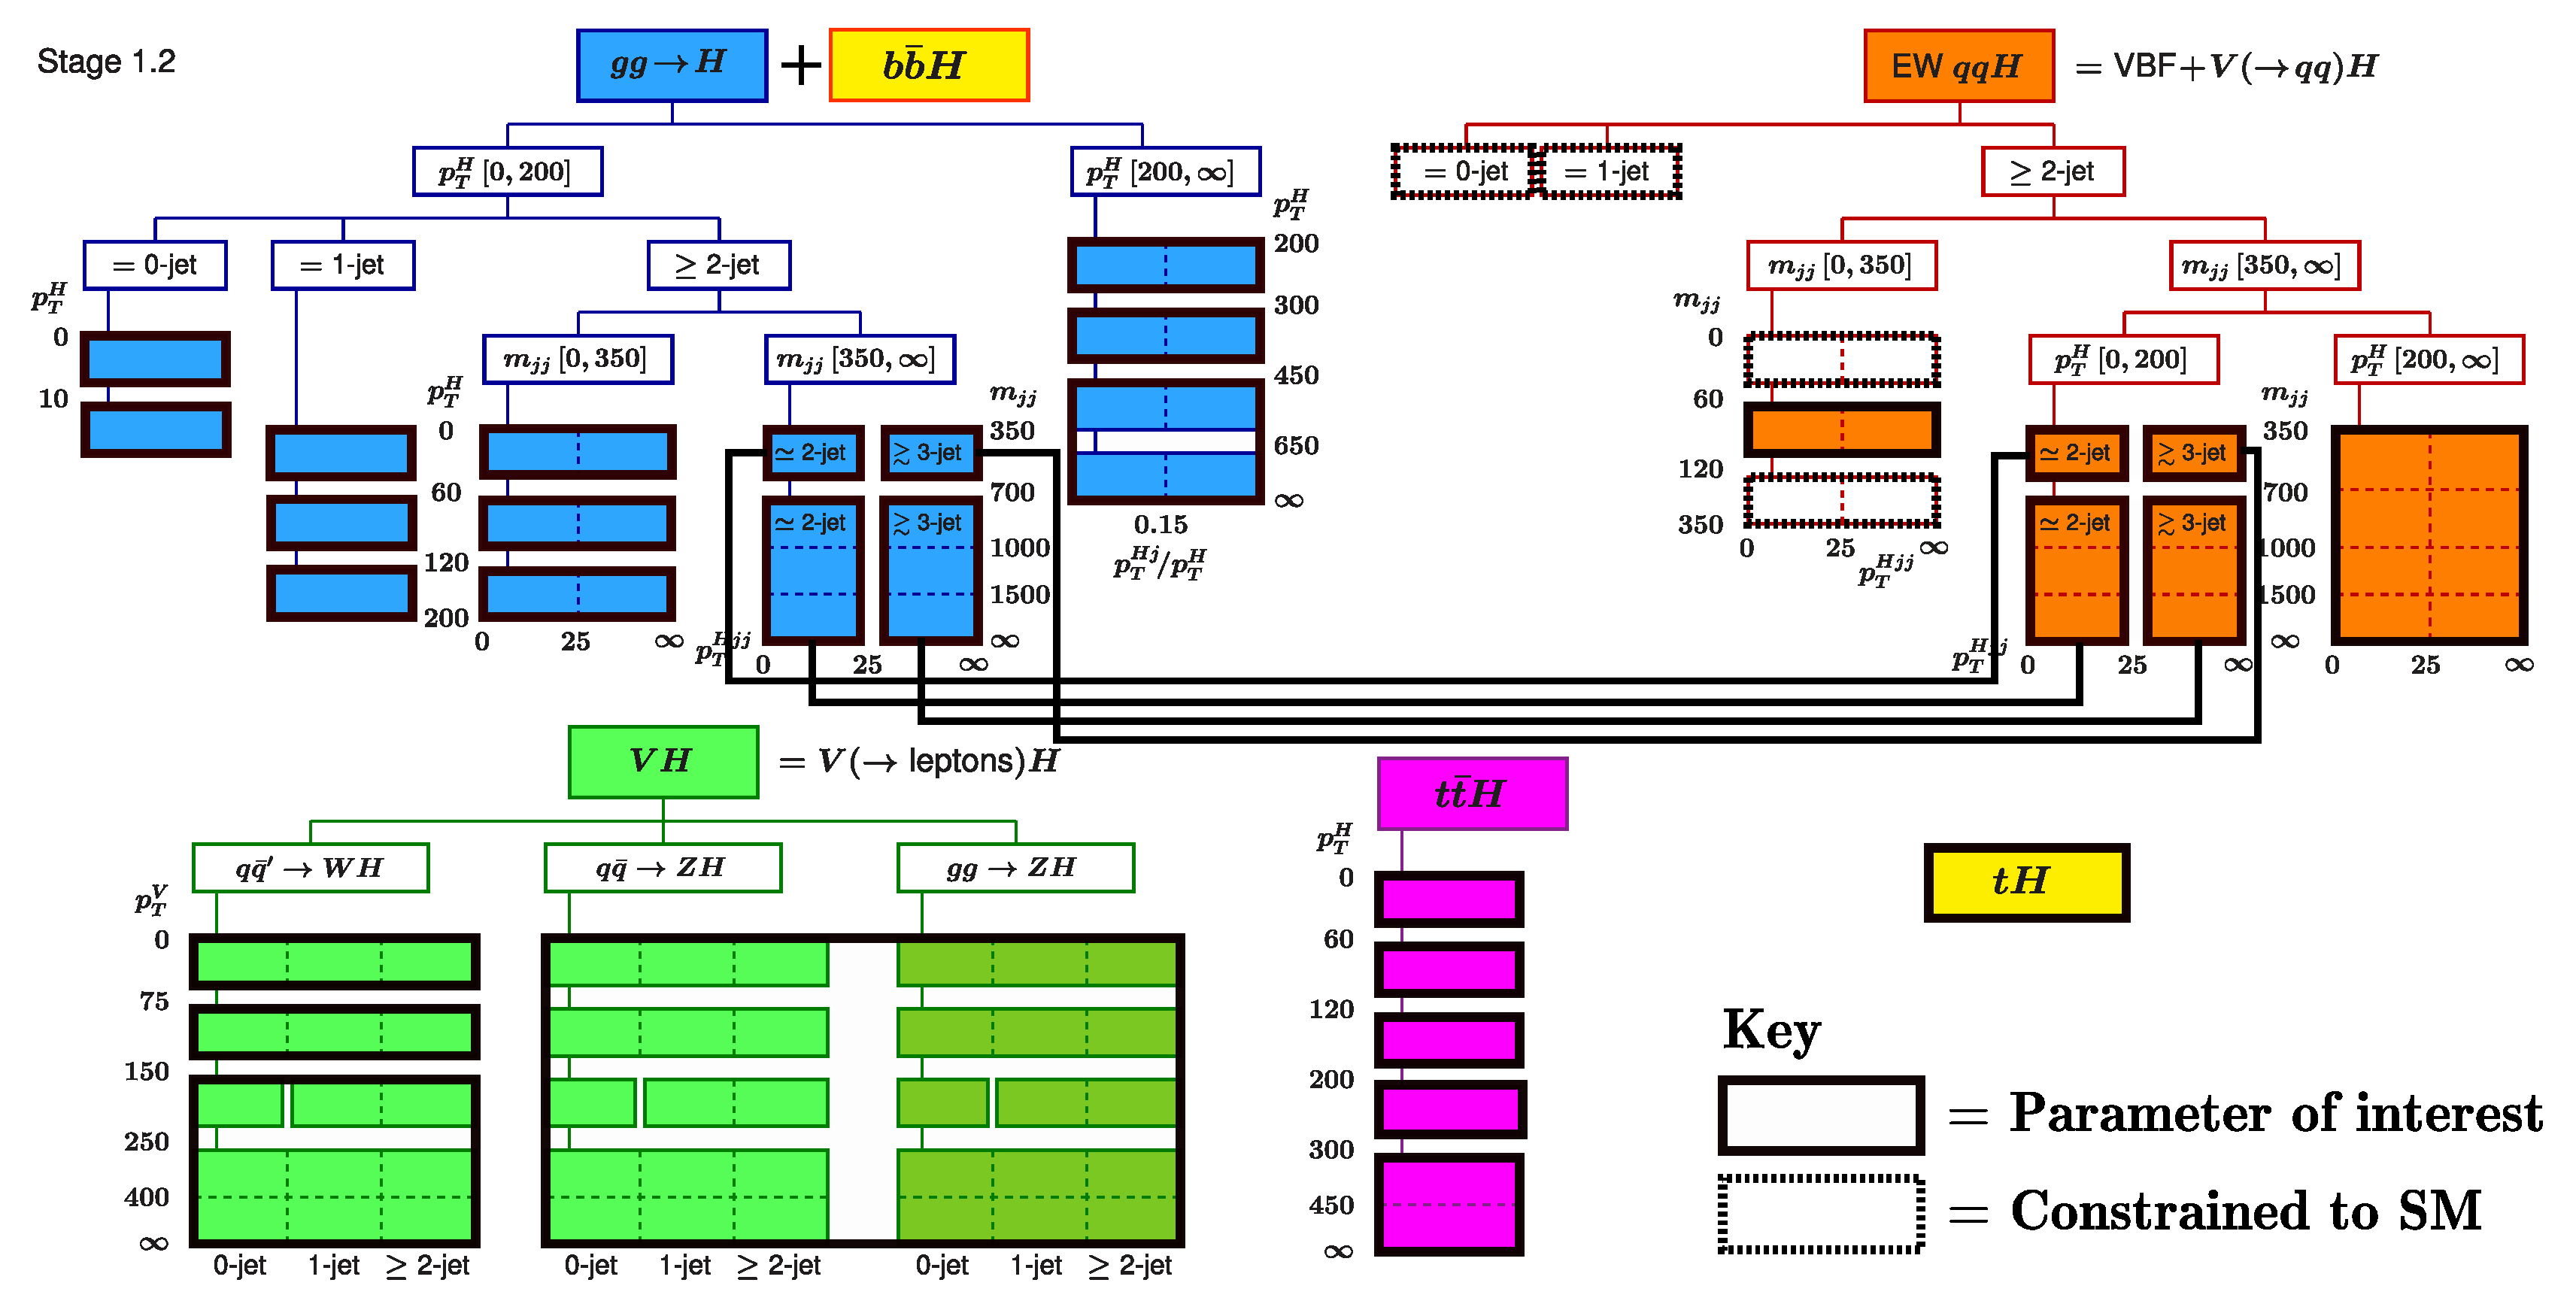
\includegraphics[width=1\linewidth]{Figures/app_merging_schemes/ms_minimal.pdf}
  \caption[Schematic of the minimal merging scheme]
  {
    Schematic to show the minimal merging scheme. The parameters of interest are defined by the solid black boxes, which span over multiple bins for the cases in which the bins are merged. The lines between the ggH VBF-like and qqH VBF-like bins indicate that these bins are merged. The hatches boxes represent the regions of phase space which are fixed to the SM prediction in the fit. In total 27 parameters of interest are defined.
  }
  \label{fig:minimal_scheme}
\end{figure}
\end{landscape}